\chapter{呼吸气体交换}\label{ch:b1:gas-exchange}

一升空气所含的氧气是一升水的三十倍，
质量轻八百倍，且氧气在其中的扩散速度
快一万倍。鳟鱼每摄取一毫克氧气，
须让一百五十克水流过其鳃，
并从中提取所携氧气的五分之四；人则
每毫克氧气需移动几克空气，并浪费其中的四分之三。
两种\omterm{def:b1:mammal-organization:organ}{器官}是同一方程——气体穿过表面的通量——
在两种介质中的两种解答。本章阐述物理原理，
推导交换表面应具备的条件，描述鳃、肺
与气管，追踪氧气与二氧化碳在血液中的转运，并
讨论通气如何受到调节，以及在高海拔
和水下\omterm{def:b1:organism-environment:organism}{环境}中会有哪些变化。

\section{气体在两种介质中的物理规律}

\begin{definition}[分压、溶解度]\label{def:b1:gas-exchange:partial}
\index{分压}
在混合气体中，每种气体各自产生一个\emph{分压}，
与其所占比例成正比：在 \qty{101}{kPa} 的空气中，氧气
（\qty{20.9}{\%}）的 $P_{\mathrm{O_2}} = \qty{21.2}{kPa}$，二氧化碳
（\qty{0.04}{\%}）为 \qty{0.04}{kPa}。气体溶于液体的量与其分压成正比
（亨利定律）：与空气处于平衡的水中，
在 \qty{15}{\celsius} 时含氧 \qty{0.32}{mmol/L}
（\qty{10}{mg/L}，\qty{7}{mL/L} 气体），而空气本身为 \qty{8.7}{mmol/L}
（\qty{210}{mL/L}）。分压——水与空气处于平衡时两者相同——
驱动了介质之间的扩散；
而含量则是呼吸者能够提取的量。二氧化碳
的溶解度是氧的二十五倍，因此它从来
不是更难交换的气体。
\end{definition}

\begin{theorem}[交换表面的菲克定律]\label{thm:b1:gas-exchange:fick}
\index{菲克定律}
气体穿过面积为 $A$、厚度为
$x$、隔开\omterm{def:b1:gas-exchange:partial}{分压}分别为 $P_1$ 与 $P_2$ 的两种介质的膜的速率为
\[
\dot V = K\,\frac{A}{x}\,(P_1 - P_2),
\]
其中 $K$ 为膜的扩散（克罗格）常数，该常数综合了
气体在\omterm{def:b1:body-plans-tissues:tissue}{组织}中的扩散性与溶解度。通量
由更大的面积、更薄的屏障及更大的\omterm{def:b1:gas-exchange:partial}{分压}差
提高，别无其他因素。
\end{theorem}
\begin{proof}
由膜中溶解气体的菲克第一定律
（见\cref{ch:b1:membranes-transport}）给出单位面积通量
与浓度梯度成正比；由亨利定律可知，
各界面处的浓度与该处介质中的\omterm{def:b1:gas-exchange:partial}{分压}成正比，
故梯度为 $(P_1 - P_2)/x$ 乘以溶解度，
常数吸收了溶解度与扩散系数。
\end{proof}

\begin{omfigure}
\begin{tikzpicture}
\begin{axis}[
  ybar, bar width=16pt,
  width=0.72\linewidth, height=5.6cm,
  axis x line=bottom, axis y line=left,
  ymode=log, log origin=infty, ymin=0.1, ymax=3000,
  ylabel={每升介质中的氧含量（\unit{mL}）},
  ylabel style={font=\small},
    symbolic x coords={air, water at 5 C, water at 15 C, water at 30 C, sea water at 15 C},
  xtick=data, xticklabels={空气, 5 °C 的水, 15 °C 的水, 30 °C 的水, 15 °C 的海水}, x tick label style={font=\small, rotate=20, anchor=north east},
  enlarge x limits=0.15,
  nodes near coords, nodes near coords style={font=\scriptsize, anchor=south},
  point meta=rawy,
]
\addplot[fill=omDef!45, draw=omDef] coordinates  {(air,210) (water at 5 C,9.0) (water at 15 C,7.1) (water at 30 C,5.3) (sea water at 15 C,5.8)};
\end{axis}
\end{tikzpicture}

{\small 空气及与其平衡的水中的氧含量。
水中的含氧量比空气少三十倍，水温升高或含盐量增大时更少：一条
夏季池塘中的鱼生活在供氧的边缘。}
\end{omfigure}

\begin{proposition}[交换表面应具备的条件]\label{prop:b1:gas-exchange:requirements}
\index{交换表面}
超过一毫米的\omterm{def:b1:organism-environment:organism}{生物体}无法单靠
通过外表面的扩散获得供应（见\cref{ch:b1:organism-environment}）。
它需要一个\emph{呼吸表面}，其面积大（以增大 $A$），
薄（以减小 $x$），湿润（气体只有溶解后才能穿过膜），
\emph{通气良好}——外部介质不断更新，使 $P_1$ 保持
较高——并且\emph{灌注良好}——其后方的血液不断更新，使
$P_2$ 保持较低；并需要循环系统将气体从表面
输送到\omterm{def:b1:body-plans-tissues:tissue}{组织}。鳃、肺和气管是三种
把此类表面折入身体并使两种流体穿过它的方式。
\end{proposition}

\section{鳃与逆流}

\begin{definition}[鳃]\label{def:b1:gas-exchange:gill}
\index{鳃}
\emph{鳃}是体表向水中的外突，
折叠成鳃丝和厚度仅数微米的\emph{鳃小片}，
血液在其中的毛细血管内流动。鱼的鳃每侧悬挂于
四根骨质鳃弓上；水从口腔吸入，
经鳃盖之下排出，借双泵系统的作用，
在鳃小片之间朝一个方向流动，而鳃小片中的血液
朝相反方向流动：形成\emph{逆流}\index{逆流交换}。
一条重一千克的鳟鱼约有 \qty{2000}{cm^2} 的鳃小片表面，
厚 \qty{2}{\micro m}。
\end{definition}

\begin{omfigure}
\begin{tikzpicture}
  \node[anchor=south west, inner sep=0] (img) at (0,0)
    {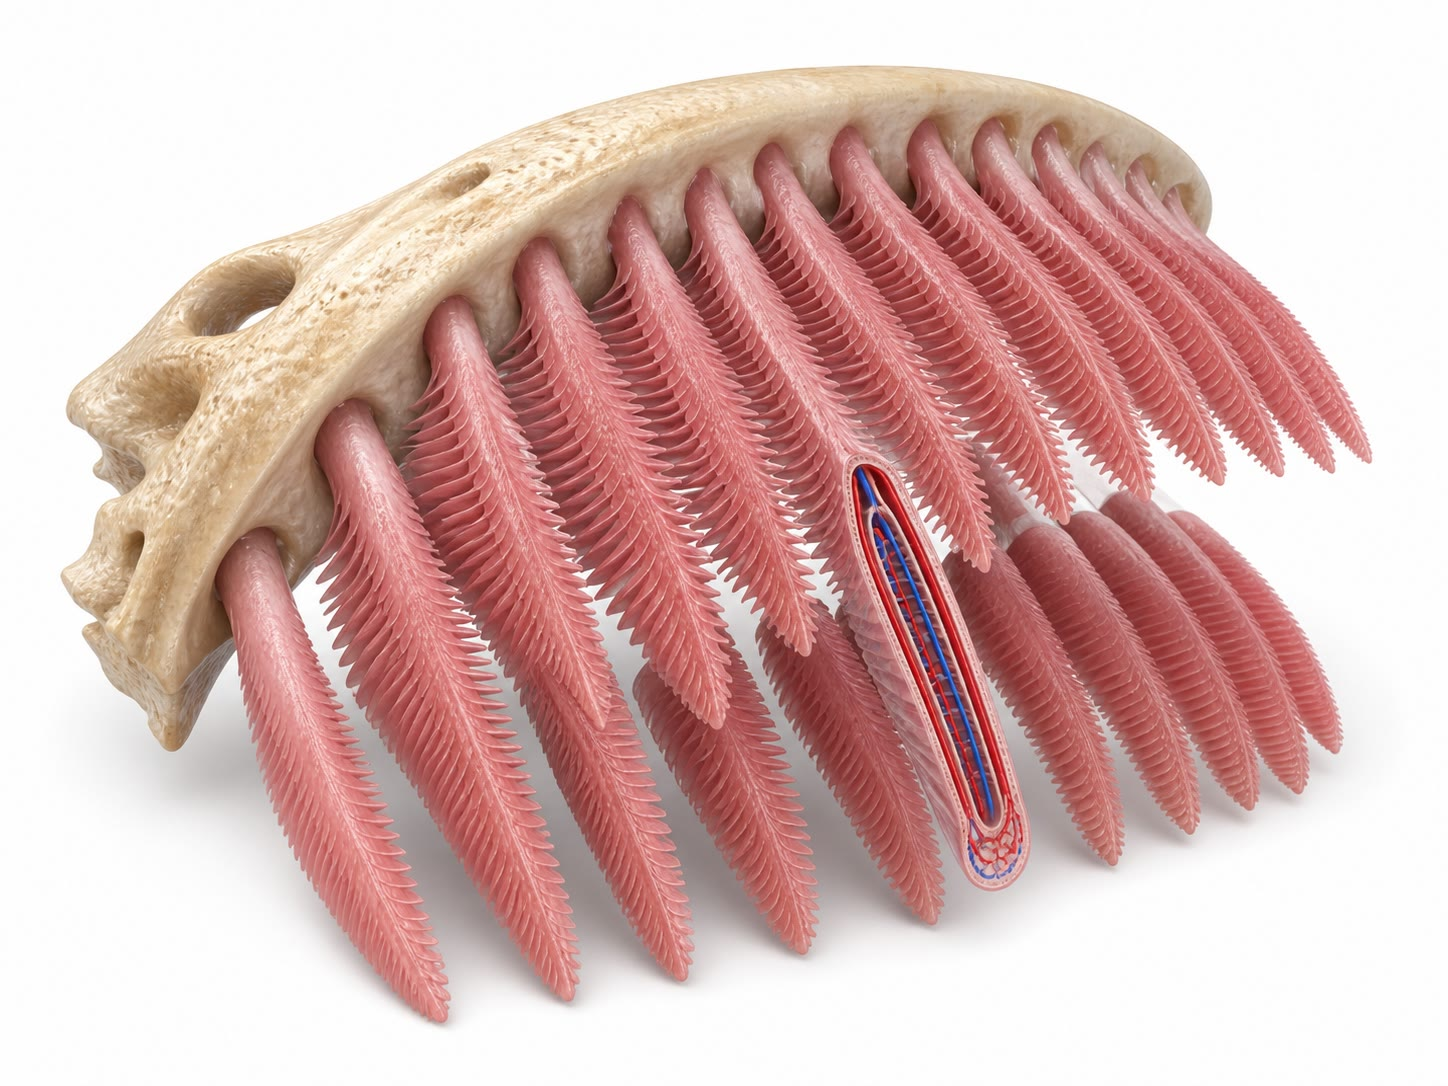
\includegraphics[width=0.52\linewidth]{images/book3/ai/fig-gill-lamellae.jpg}};
  \begin{scope}[x={(img.south east)}, y={(img.north west)},
      every node/.style={font=\small}]
    \draw[omDef, thick] (0.20,0.50) -- (-0.03,0.60) node[left] {鳃弓};
    \draw[omDef, thick] (0.55,0.70) -- (0.55,1.08) node[above] {鳃丝};
    \draw[omDef, thick] (0.75,0.40) -- (1.03,0.30) node[right, align=left] {鳃小片：交换表面，\\ 厚 \qty{2}{\micro m}};
    \draw[omDef, thick] (0.45,0.20) -- (0.45,-0.08) node[below] {沿鳃丝的血管};
  \end{scope}
\end{tikzpicture}

{\small 一个鳃弓连同其鳃丝及鳃小片。水
在鳃小片之间流动，血液则以相反方向流过它们。}
\end{omfigure}

\begin{theorem}[逆流交换]\label{thm:b1:gas-exchange:countercurrent}
当水与血液沿一交换表面以相反方向流动时，
离开鳃的血液可以接近
\emph{进入}鳃的水的\omterm{def:b1:gas-exchange:partial}{分压}，水中大部分的
氧可以被夺去，提取率可达 \qty{80}{\%} 或更高。当二者
同向流动时（顺流），两种流体都趋向一个共同的中间值，
提取率不能超过 \qty{50}{\%}。
\end{theorem}
\begin{proof}
在顺流交换器中，差值 $P_{\text{水}} -
P_{\text{血液}}$ 从入口值降为零，即两者
趋于相同的压强；一旦二者相等，便不再有气体移动，
且在流量相等时，相遇点恰在中点。在\omterm{def:b1:gas-exchange:gill}{逆流}中，
血液向其出口流动时，会遇到越来越新鲜的水，
因此整个长度上都保持正的压差，
血液在出口处面对的是 \qty{21}{kPa} 的入水，
水在出口处面对的是仅几千帕的入流静脉血，
极限由交换表面决定，而非由平衡决定。
\end{proof}

\begin{omfigure}
\begin{tikzpicture}[font=\footnotesize, >=Stealth, line cap=round]
  % co-current
  \begin{scope}
    \node[anchor=south, font=\small] at (2.6,1.65) {顺流：两股流体同向};
    \draw[->, very thick, omDef] (0,1.2) -- (5.2,1.2) node[right] {水出口：\qty{12}{kPa}};
    \draw[->, very thick, omThm] (0,0.4) -- (5.2,0.4) node[right] {血液出口：\qty{12}{kPa}};
    \node[anchor=east, omDef] at (-0.1,1.2) {水入口：\qty{21}{kPa}};
    \node[anchor=east, omThm] at (-0.1,0.4) {血液入口：\qty{3}{kPa}};
    \foreach \x/\d in {0.6/18, 1.6/12, 2.6/7, 3.6/3, 4.6/0.5} { \draw[->, gray] (\x,1.05) -- (\x,0.55) node[midway, right, font=\scriptsize, gray] {\d}; }
    \node[anchor=north, align=center] at (2.6,0.1) {差值（灰色，kPa）减小至零：\\ 提取止于 \qty{43}{\%}};
  \end{scope}
  \begin{scope}[yshift=-3.6cm]
    \node[anchor=south, font=\small] at (2.6,1.65) {逆流：两股流体反向};
    \draw[->, very thick, omDef] (0,1.2) -- (5.2,1.2) node[right] {水出口：\qty{4}{kPa}};
    \draw[<-, very thick, omThm] (0,0.4) -- (5.2,0.4) node[right] {血液入口：\qty{3}{kPa}};
    \node[anchor=east, omDef] at (-0.1,1.2) {水入口：\qty{21}{kPa}};
    \node[anchor=east, omThm] at (-0.1,0.4) {血液出口：\qty{18}{kPa}};
    \foreach \x/\d in {0.6/3, 1.6/3, 2.6/3, 3.6/3, 4.6/2} { \draw[->, gray] (\x,1.05) -- (\x,0.55) node[midway, right, font=\scriptsize, gray] {\d}; }
    \node[anchor=north, align=center] at (2.6,0.1) {差值沿全程保持为正：\\ 提取率达 \qty{80}{\%}，血液离开时接近水的入口值};
  \end{scope}
\end{tikzpicture}

{\small 顺流与\omterm{def:b1:gas-exchange:gill}{逆流交换}，交换表面与流量相同。
逆向流动使整个长度上都保持梯度，
并使血液接近新鲜水的氧
\omterm{def:b1:gas-exchange:partial}{分压}。}
\end{omfigure}

\begin{omfigure}
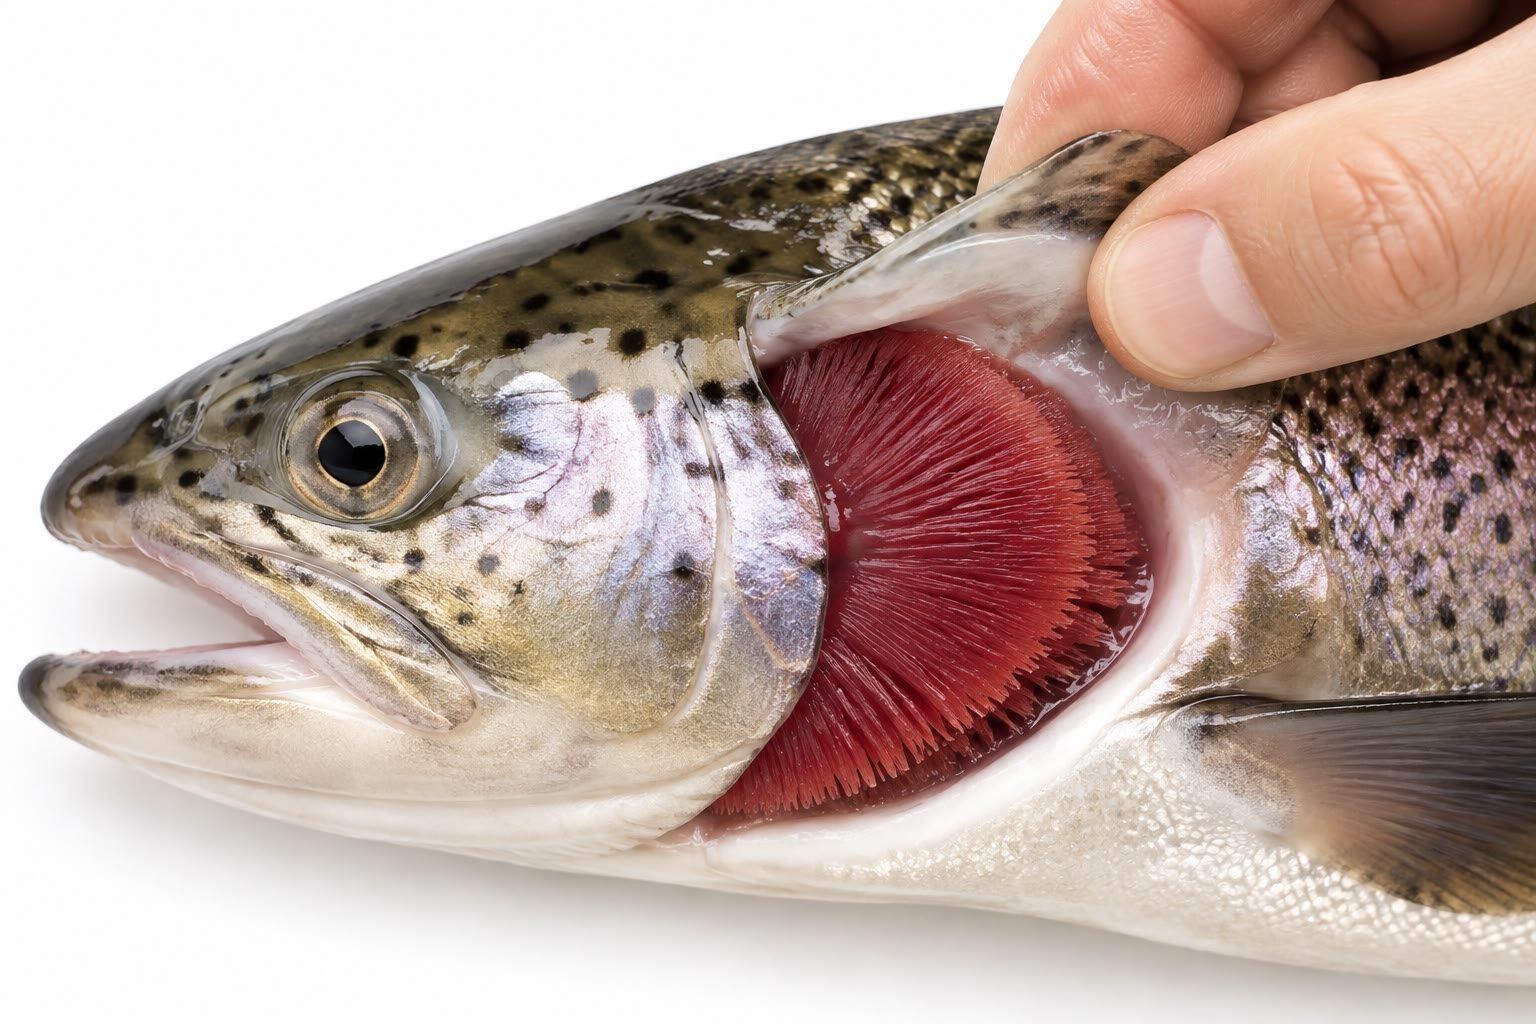
\includegraphics[width=0.5\linewidth]{images/book3/ai/b3-21-trout-gills.jpg}

{\small 鳟鱼掀起鳃盖后露出的鳃：呈红色，
因为鳃小片只有两个\omterm{def:b1:cell-unit-of-life:cell}{细胞}厚，血液
与水仅相距一微米。}
\end{omfigure}

\begin{example}[水的代价]\label{ex:b1:gas-exchange:priceofwater}
一条静息的 \qty{1}{kg} 鳟鱼每小时约摄取 \qty{50}{mL} 氧气。
从含氧 \qty{7}{mL/L} 的水中提取，提取率为 \qty{80}{\%}，它每小时须
泵送 \qty{9}{L} 水流过鳃——九千克黏度比空气高五十倍的介质，流经
宽度不足一毫米的通道。它的代谢有十分之一用于呼吸；静息的
人则只用五十分之一。若把池塘加热到 \qty{30}{\celsius}，
同一条鱼需从含氧更低的水中获取更多的氧，
因此须泵送三倍的水量。
因此须泵送三倍的水量。
\end{example}

\section{呼吸空气：肺与气管}

\begin{definition}[哺乳动物的肺]\label{def:b1:gas-exchange:lung}
\index{肺}\index{肺泡}
称\emph{肺}为体表向体内凹陷而成的湿润
内腔，使该表面在干燥空气中保持湿润。哺乳动物的
肺是由气道构成的树，末端连接约三亿个
\emph{肺泡}，为直径 \qty{0.2}{mm} 的小囊，其壁由
一层\omterm{def:b1:body-plans-tissues:epithelium}{上皮}\omterm{def:b1:cell-unit-of-life:cell}{细胞}与一层毛细血管内皮构成，二者合计厚度 \qty{0.5}{\micro m}，
其总面积在人体中达 \qty{100}{m^2}，外包
一张毛细血管网，全部心输出量都流经其中。肺以
\emph{潮式}通气：\omterm{def:b1:mammal-organization:bodyplan}{膈肌}与肋间肌使胸腔扩大，空气
流入；它们舒张时，空气沿原路流出。一次
呼吸移动 \qty{500}{mL} 气体，其中 \qty{150}{mL} 仅充满气道
（\emph{无效腔}）从未到达任何肺泡；肺泡气，
每次呼吸更新其七分之一，保持在 $P_{\mathrm{O_2}} =
\qty{13.3}{kPa}$ 与 $P_{\mathrm{CO_2}} = \qty{5.3}{kPa}$，即
血液与之达到平衡的\omterm{def:b1:gas-exchange:partial}{分压}。
\end{definition}

\begin{omfigure}
\begin{tikzpicture}
  \node[anchor=south west, inner sep=0] (img) at (0,0)
    {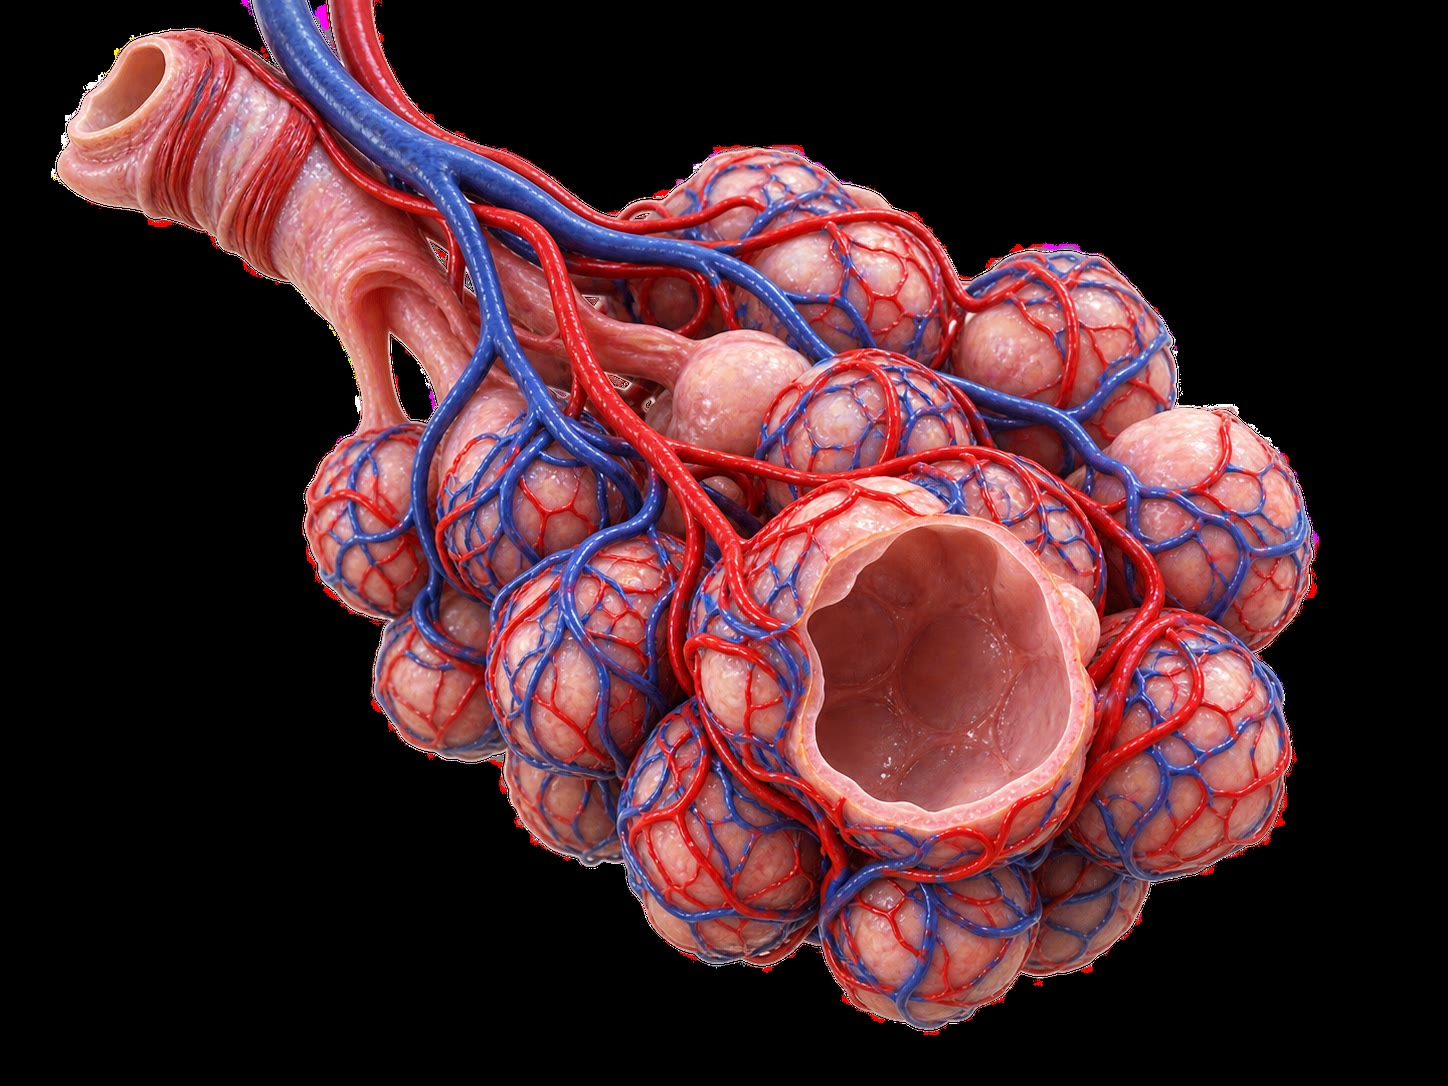
\includegraphics[width=0.5\linewidth]{images/book3/ai/fig-alveoli.jpg}};
  \begin{scope}[x={(img.south east)}, y={(img.north west)},
      every node/.style={font=\small}]
    \draw[omDef, thick] (0.50,0.85) -- (0.50,1.08) node[above] {末端气道};
    \draw[omDef, thick] (0.30,0.45) -- (-0.03,0.40) node[left, align=right] {切开的肺泡：\\ 内含空气};
    \draw[omDef, thick] (0.75,0.55) -- (1.03,0.62) node[right, align=left] {毛细血管网 \\ 位于壁上};
    \draw[omDef, thick] (0.60,0.15) -- (0.60,-0.08) node[below] {肺泡壁：空气与血液之间 \qty{0.5}{\micro m}};
  \end{scope}
\end{tikzpicture}

{\small 气道末端的\omterm{def:b1:gas-exchange:lung}{肺泡}，外包毛细血管。全部
心输出量分布于这层壁的一百平方米上，
每次仅历时一秒的一小部分。}
\end{omfigure}

\begin{proposition}[空气的三种设计]\label{prop:b1:gas-exchange:designs}
\index{气管}
\emph{哺乳动物}采用潮式通气：结构简单，但新鲜空气会与
陈旧空气混合，\omterm{def:b1:gas-exchange:lung}{肺泡}氧含量为大气的三分之二，
提取率则为四分之一。\emph{鸟类}使空气沿单一方向
穿过位于两组充当风箱的气囊之间的细管，
使新鲜空气流经交换面，
吸气和呼气时均如此，与血液呈交叉\omterm{def:b1:gas-exchange:gill}{逆流}，
其提取率更高，斑头雁能飞越喜马拉雅山，
而哺乳动物在那里会昏厥。\emph{昆虫}根本没有
呼吸用血液：空气经瓣膜（\emph{气门}）
进入\emph{气管}，这些管道由螺旋状加厚结构撑开，
分支可细至微米级，经扩散直接把氧气送到
每一个\omterm{def:b1:cell-unit-of-life:cell}{细胞}；在大型或活动强烈的
昆虫中，还借助腹部的泵动。沿管道的扩散将这一设计限于小体形——
这也是没有昆虫比老鼠更大的原因之一。
\end{proposition}

\begin{omfigure}
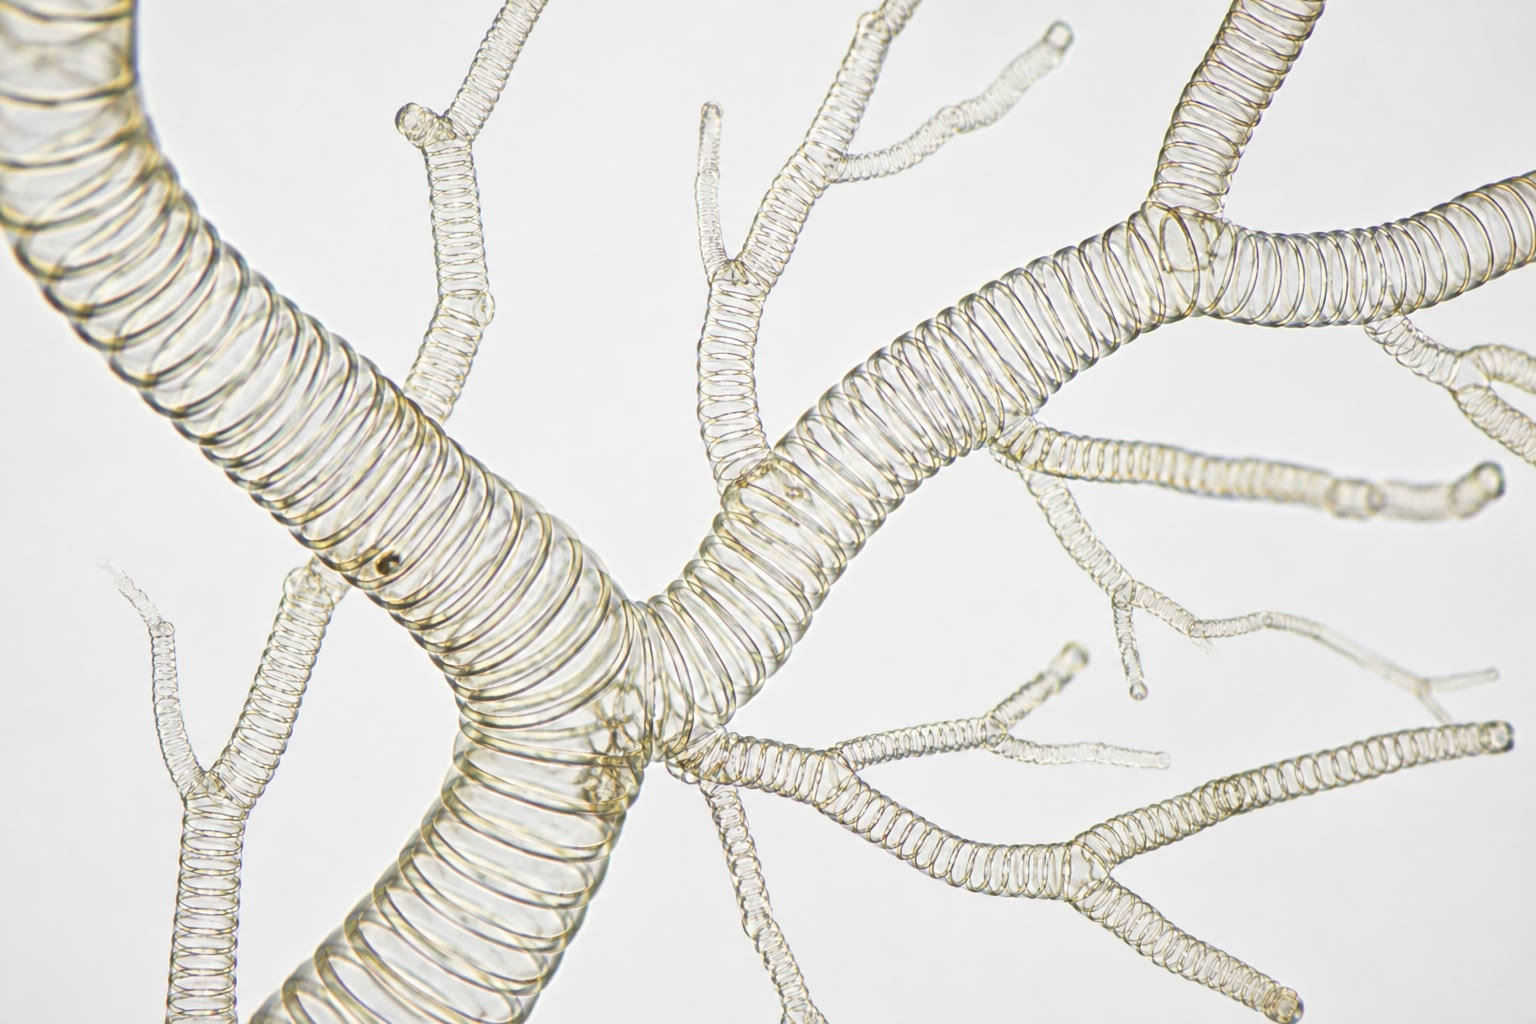
\includegraphics[width=0.5\linewidth]{images/book3/ai/b3-21-insect-tracheae.jpg}

{\small 昆虫气管：充满空气的管道，由螺旋状加厚结构撑开，
分支一直延伸到\omterm{def:b1:cell-unit-of-life:cell}{细胞}。没有血液运载氧气；
空气一直送到\omterm{def:b1:cell-unit-of-life:cell}{细胞}处。}
\end{omfigure}

\begin{method}[读懂通气收支]\label{met:b1:gas-exchange:budget}
\begin{enumerate}
  \item 每分钟通气量 $=$ 潮气量 $\times$ 每
        分钟呼吸次数；\omterm{def:b1:gas-exchange:lung}{肺泡}通气量 $=$ （潮气量 $-$ 无效腔）
        $\times$ 每分钟呼吸次数。只有后者才发生气体交换。
  \item 氧摄取量 $=$ \omterm{def:b1:gas-exchange:lung}{肺泡}通气量 $\times$ （吸入气中
        氧分数 $-$ \omterm{def:b1:gas-exchange:lung}{肺泡}气中氧分数）；静息时，
        $\qty{4.2}{L/min}\times(0.21 - 0.14) \approx \qty{0.3}{L/min}$。
  \item 提取率 $=$ 摄取量 $/$ （通气量 $\times$ 吸入气
        氧分数）：潮式通气的肺中为四分之一，
        在\omterm{def:b1:gas-exchange:gill}{逆流}式鳃中为五分之四。
  \item 从血液一侧看：摄取量 $=$ 心输出量 $\times$
        （动脉血含量 $-$ 静脉血含量）；\qty{5}{L/min}$\times$
        \qty{50}{mL/L}，静息时同为 \qty{250}{mL/min}。两份
        收支必须一致。
\end{enumerate}
\end{method}

\section{血液中的气体}

\begin{proposition}[氧气与二氧化碳的运输]\label{prop:b1:gas-exchange:transport}
\index{碳酸酐酶}\index{玻尔效应}\index{霍尔丹效应}
\omterm{def:b1:mammal-organization:compartments}{血浆}在动脉压下每升仅溶解 \qty{3}{mL} 氧气；
血红蛋白（\cref{ch:b1:proteins}）携带 \qty{200}{mL} 氧气，
在肺中于 \qty{13.3}{kPa} 下结合，在\omterm{def:b1:body-plans-tissues:tissue}{组织}中释放五分之一至
一半。二氧化碳有三种运输方式：\qty{7}{\%}
溶解态，\qty{23}{\%} 与血红蛋白的氨基结合，并且
\qty{70}{\%} 以碳酸氢根形式存在：在红\omterm{def:b1:cell-unit-of-life:cell}{细胞}中，\emph{\omterm{prop:b1:gas-exchange:transport}{碳酸
酐酶}}将 $\mathrm{CO_2}$ 与水在
数毫秒内转化为碳酸；碳酸解离，碳酸氢根离开\omterm{def:b1:cell-unit-of-life:cell}{细胞}，
以氯离子进入作为交换（即\emph{氯离子转移}），质子则
被血红蛋白摄取。两种气体相互促进：酸与
$\mathrm{CO_2}$ 降低血红蛋白对氧的亲和力（\emph{\omterm{prop:b1:gas-exchange:transport}{玻尔
效应}}），使氧在 $\mathrm{CO_2}$ 生成处释放；而
去氧血红蛋白结合质子和 $\mathrm{CO_2}$ 的能力更强
（\emph{\omterm{prop:b1:gas-exchange:transport}{霍尔丹效应}}），故 $\mathrm{CO_2}$ 在氧释放处被摄取，
并在肺中随着氧的结合而释出。
\end{proposition}

\begin{omfigure}
\begin{tikzpicture}[font=\footnotesize, >=Stealth, line cap=round]
  % red cell
  \draw[very thick, omThm!80!black, fill=omThm!8, rounded corners=18pt] (0,0) rectangle (7.6,4.0);
  \node[anchor=north west, omThm!80!black, font=\small] at (0.15,3.95) {红细胞（位于组织毛细血管中）};
  % CO2 in from tissue
  \draw[->, very thick, omDef] (-1.6,2.6) -- (0,2.6) node[pos=0, left, align=right] {$\mathrm{CO_2}$ 来自 \\ 组织};
  \node[draw, thick, fill=white, rounded corners=3pt, inner sep=2pt] (ca) at (2.0,2.6) {$\mathrm{CO_2} + \mathrm{H_2O} \to \mathrm{H_2CO_3}$};
  \node[anchor=south, font=\scriptsize, omProp!80!black] at (2.0,2.95) {碳酸酐酶};
  \node[draw, thick, fill=white, rounded corners=3pt, inner sep=2pt] (dis) at (5.2,2.6) {$\mathrm{H^+} + \mathrm{HCO_3^-}$};
  \draw[->, thick] (ca) -- (dis);
  % bicarbonate out, chloride in
  \draw[->, very thick, omDef] (6.2,2.4) -- (6.2,0.9) -- (8.4,0.9) node[right, align=left] {$\mathrm{HCO_3^-}$ 进入血浆 \\（\qty{70}{\%} 的 $\mathrm{CO_2}$）};
  \draw[<-, very thick, gray] (6.9,1.85) -- (8.4,1.85) node[right, gray] {$\mathrm{Cl^-}$ 交换进入};
  % proton to Hb, O2 release
  \node[draw, thick, fill=omThm!25, rounded corners=3pt, inner sep=2pt] (hb) at (4.0,1.0) {血红蛋白};
  \draw[->, thick] (4.7,2.35) -- (4.2,1.3) node[midway, right, font=\scriptsize] {$\mathrm{H^+}$ 结合};
  \draw[->, very thick, omExo!70!black] (hb.west) -- (0,1.0) -- (-1.6,1.0) node[left, align=right] {$\mathrm{O_2}$ 释放 \\（玻尔效应）};
  \node[anchor=north, align=center, gray] at (3.8,-0.2) {在肺中每个箭头方向相反：氧结合，质子与 $\mathrm{CO_2}$ 被释放，\\ 碳酸氢根重新进入细胞，$\mathrm{CO_2}$ 被呼出};
\end{tikzpicture}

{\small 红\omterm{def:b1:cell-unit-of-life:cell}{细胞}中的二氧化碳。\omterm{prop:b1:gas-exchange:transport}{碳酸酐酶}催化生成
碳酸；碳酸氢根进入\omterm{def:b1:mammal-organization:compartments}{血浆}，质子则
被血红蛋白结合，血红蛋白同时释放氧。}
\end{omfigure}

\begin{example}[一升血液流经工作中的肌肉]\label{ex:b1:gas-exchange:litre}
动脉血每升携带 \qty{200}{mL} 氧气，并
携带 \qty{480}{mL} 二氧化碳（大部分以碳酸氢根形式存在）。在静息
时的肌肉中，血液离开时仍含 \qty{50}{mL} 氧气，并摄取 \qty{40}{mL} 的
$\mathrm{CO_2}$；静脉血 \omterm{def:b1:water-small-molecules:ph}{pH} 仅下降 \qty{0.04}{}，因为
血红蛋白已吸收了质子。在短跑时的肌肉中，\omterm{def:b1:water-small-molecules:ph}{pH}
为 7.2，$P_{\mathrm{O_2}}$ 为 \qty{2.7}{kPa}，同一升血液离开时
仍含 \qty{150}{mL} 氧气（\cref{ch:b1:proteins}），并
也带走了乳酸。
\end{example}

\section{呼吸调控、高海拔与潜水}

\begin{proposition}[通气受二氧化碳调控]\label{prop:b1:gas-exchange:control}
\index{化学感受器}
呼吸节律由脑干产生，并受
\emph{化学感受器}调节：中枢化学感受器浸浴于脑周围的液体中，
对 $\mathrm{CO_2}$ 产生的 \omterm{def:b1:water-small-molecules:ph}{pH} 变化作出反应；
外周化学感受器位于颈动脉，对动脉血氧
\omterm{def:b1:gas-exchange:partial}{分压}降至约 \qty{8}{kPa} 以下时作出反应。日常生活中起主导作用的是
$\mathrm{CO_2}$：动脉血
$P_{\mathrm{CO_2}}$ 升高 \qty{1}{kPa}，通气量约加倍，而氧
须下降三分之一，通气才有反应。屏气何时结束，
取决于 $\mathrm{CO_2}$（而非氧）达到极限；过度通气先
降低 $\mathrm{CO_2}$，使潜水者得以在水下停留，直到氧耗尽
为止——在呼吸冲动恢复之前已经失去意识。
\end{proposition}

\begin{omfigure}
\begin{tikzpicture}
\begin{axis}[
  width=0.86\linewidth, height=5.8cm,
  axis x line=bottom, axis y line=left,
  xmin=4, xmax=8.5, ymin=0, ymax=45,
  xlabel={动脉血 $P_{\mathrm{CO_2}}$ (\unit{kPa})}, ylabel={通气量 (\unit{L/min})},
  xlabel style={font=\small, at={(axis description cs:0.5,-0.13)}, anchor=north},
  ylabel style={font=\small},
  tick label style={font=\small}, xtick={4,5,6,7,8}, ytick={0,10,20,30,40},
  legend style={font=\small, at={(0.03,0.97)}, anchor=north west, draw=none},
  clip=false,
]
\addplot[very thick, omDef, domain=4.5:8.5, samples=20] {6 + 10*(x-5.3)};
\addlegendentry{正常氧分压}
\addplot[very thick, omThm, domain=4.5:7.2, samples=20] {6 + 20*(x-5.3)};
\addlegendentry{低氧（\qty{7}{kPa}）：斜率更大}
\draw[dashed, gray] (axis cs:5.3,0) -- (axis cs:5.3,6); \node[font=\scriptsize, anchor=west] at (axis cs:5.4,1.5) {静息值};
\end{axis}
\end{tikzpicture}

{\small 通气量与动脉血二氧化碳\omterm{def:b1:gas-exchange:partial}{分压}的关系。高于静息值每 \qty{1}{kPa}，
通气量约增加 \qty{10}{L/min}；低氧使反应曲线变陡，
但单独存在时，只有在严重时才有明显影响。}
\end{omfigure}

\begin{example}[海拔与潜水]\label{ex:b1:gas-exchange:altitudediving}
在 \qty{4000}{m} 处，空气中的氧\omterm{def:b1:gas-exchange:partial}{分压}为 \qty{12}{kPa}，\omterm{def:b1:gas-exchange:lung}{肺泡}中的
氧\omterm{def:b1:gas-exchange:partial}{分压}为 \qty{7}{}：颈动脉体推动通气加强，这会排出 
$\mathrm{CO_2}$，使血液碱化——这是一种制动机制，肾脏
通过排出碳酸氢盐，在数日内将其解除；红\omterm{def:b1:cell-unit-of-life:cell}{细胞}在数日内提高其 
BPG 含量，骨髓则在数周内提高血红蛋白水平
（见\cref{ch:b1:proteins}）。海豹潜水二十分钟时，情况恰好相反：它在下潜前先呼出气体，
将心率降至十分之一，阻断
除大脑和心脏以外各处的血液供应，其肌肉则
依靠与自身肌红蛋白结合的氧运转，肌红蛋白浓度为人的十倍，
随后转为\omterm{def:b1:respiration-fermentation:fermentation}{发酵}供能，并耐受乳酸，乳酸
在浮出水面后被机体清除。其肺在 \qty{50}{m} 以下
会塌陷，从而阻止氮气进入血液。
\end{example}

\section{练习}

\begin{exercise}[$\star$]\label{exo:b1:gas-exchange:1}
写出交换表面的菲克定律，
并列出使通量增大的四个特征。
\end{exercise}

\begin{exercise}[$\star$]\label{exo:b1:gas-exchange:2}
解释为何水比空气更难用于呼吸，
并用三个数值加以说明。
\end{exercise}

\begin{exercise}[$\star$]\label{exo:b1:gas-exchange:3}
由\omterm{def:b1:gas-exchange:gill}{逆流}示意图读出每种排列中流出的水的氧\omterm{def:b1:gas-exchange:partial}{分压}，
以及流出的血液的氧\omterm{def:b1:gas-exchange:partial}{分压}，
并读出提取率。
\end{exercise}

\begin{exercise}[$\star$]\label{exo:b1:gas-exchange:4}
二氧化碳以哪三种形式在血液中运输，
各占的比例是多少？
\end{exercise}

\begin{exercise}[$\star\star$]\label{exo:b1:gas-exchange:5}
某人每分钟呼吸 \qty{15}{} 次，潮气量为
\qty{450}{mL}，无效腔为 \qty{150}{mL}。计算每分通气量与\omterm{def:b1:gas-exchange:lung}{肺泡}通气量，
以及氧的摄取量，设\omterm{def:b1:gas-exchange:lung}{肺泡}中的氧分数为 
\qty{14}{\%}。若改为 \qty{30}{} 次浅呼吸，每次 \qty{225}{mL}，重复上述计算。
\end{exercise}

\begin{exercise}[$\star\star$]\label{exo:b1:gas-exchange:6}
在 \qty{25}{\celsius} 时，金鱼缸中的水每升含
\qty{6}{mL} 氧气。一条 \qty{20}{g} 的鱼每小时耗氧 \qty{2}{mL}。
在提取率为 \qty{75}{\%} 时，它的鳃每小时必须让多少水通过，
这相当于其自身体积的多少倍？
\end{exercise}

\begin{exercise}[$\star\star$]\label{exo:b1:gas-exchange:7}
一个面积为 \qty{100}{m^2}、厚度为 \qty{0.5}{\micro m} 的肺，
在平均压差为 \qty{8}{kPa} 时，每分钟转运 \qty{250}{mL/min}。
某疾病使壁增厚至 \qty{2}{\micro m}，并使面积减半。
在相同压差下计算转运量，并计算
恢复到 \qty{250}{mL/min} 所需的压差。为什么机体不能
简单地提高压差？
\end{exercise}

\begin{exercise}[$\star\star$]\label{exo:b1:gas-exchange:8}
解释氯离子转移：为何碳酸氢根离开红\omterm{def:b1:cell-unit-of-life:cell}{细胞}，为何
氯离子进入，以及没有这一交换时\omterm{def:b1:cell-unit-of-life:cell}{细胞}的
体积会发生什么变化。
\end{exercise}

\begin{exercise}[$\star\star$]\label{exo:b1:gas-exchange:9}
为何在屏气潜水前过度通气的潜水者有溺水风险，
而未过度通气者能安全浮出水面，虽然不适，
但仍保持清醒？
\end{exercise}

\begin{exercise}[$\star\star\star$]\label{exo:b1:gas-exchange:10}
一条长 \qty{1}{mm}、直径 \qty{20}{\micro m} 的昆虫气管
为一块肌肉供氧，该肌肉每秒耗氧 \qty{1e-9}{mol}。
已知空气中 $D = \qty{2e-5}{m^2/s}$，
气门处的氧浓度为 \qty{8.7}{mol/m^3}，计算肌肉端的浓度（菲克定律：
$J = DA\,\Delta c/L$）。若气管长 \qty{10}{mm}，重复上述计算。
昆虫的体型受什么限制？
\end{exercise}

\begin{exercise}[$\star\star\star$]\label{exo:b1:gas-exchange:11}
鸟类和鱼类利用的都是非潮式的流动。比较它们的
交换器（介质的流向、与血流的关系，
以及提取率），并解释为何潮式肺无论表面积多大，
都无法达到它们的提取率。
\end{exercise}

\begin{exercise}[$\star\star\star$]\label{exo:b1:gas-exchange:12}
“肺受其所排出的气体调节，
而非受其所吸入的气体调节。”用一段话讨论：为何在海平面上 $\mathrm{CO_2}$ 是更好的
信号，这一安排何时失效，以及海拔高度如何
暴露它。
\end{exercise}

\section{问题：鳟鱼与人}

\begin{problem}[{周末问题——鳃与肺并列比较：
每升介质中的氧气、通气与提取、
逆流与潮式流动，以及各自背后的血液，
最后归结为逆流鳃的提取效率}]
\label{pb:b1:gas-exchange:1}
静息状态下的成年人每分钟摄入 \qty{250}{mL} 氧气，呼吸
\qty{12}{} 次每分钟，潮气量为 \qty{500}{mL}，无效腔为
\qty{150}{mL}；吸入空气含氧 \qty{21}{\%}，\omterm{def:b1:gas-exchange:lung}{肺泡}气含氧
\qty{14}{\%}；心输出量为 \qty{5}{L/min}，动脉血含氧量为
\qty{200}{mL/L}。静息状态下、体重 \qty{1}{kg} 的鳟鱼，
每小时摄入 \qty{50}{mL} 氧气，所处水温为 \qty{15}{\celsius}，
含氧 \qty{7}{mL/L}；其血红蛋白饱和时可携带 \qty{100}{mL/L}；
其血液离开鳃时饱和度为 \qty{95}{\%}，返回时为
\qty{15}{\%}。水的密度是空气的 \qty{800}{} 倍。

\medskip
\noindent\textbf{第一部分——两种介质。}
\begin{enumerate}
  \item 以毫摩尔每升表示空气及鳟鱼所处水中的氧含量
        （\qty{22.4}{L/mol}）。
  \item 计算两者含量之比。
  \item 计算携带 \qty{1}{mmol} 氧气所需介质的质量（空气 \qty{1.2}{g/L}；
        水 \qty{1000}{g/L}），
        分别对两种情形求出。
  \item 计算能携带与一升空气等量氧气的鳟鱼用水
        的体积。
  \item 用一句话解释为何鱼鳃必须单向通气，
        而肺可以是潮式的。
\end{enumerate}

\medskip
\noindent\textbf{第二部分——肺。}
\begin{enumerate}[resume]
  \item 计算每分钟通气量与\omterm{def:b1:gas-exchange:lung}{肺泡}通气量。
  \item 每次呼吸中无效腔所占的比例为多少，
        因此每分钟通气量中有多大比例被浪费？
  \item 计算每分钟输送至\omterm{def:b1:gas-exchange:lung}{肺泡}的氧气量，以及
        被摄取的氧气量（\omterm{def:b1:gas-exchange:lung}{肺泡}通气量 $\times$
        分数之差），并与 \qty{250}{mL/min} 进行核对。
  \item 计算提取效率：摄取量除以
        每分钟吸入气体中的氧气量。
  \item 由\omterm{def:b1:gas-exchange:lung}{肺泡}气中的氧分数计算\omterm{def:b1:gas-exchange:lung}{肺泡} $P_{\mathrm{O_2}}$
        （总压 \qty{101}{kPa}，须先减去
        \qty{6.3}{kPa} 的水蒸气\omterm{def:b1:gas-exchange:partial}{分压}）。
  \item 在血液一侧，计算心输出量为 \qty{5}{L/min} 时
        摄取 \qty{250}{mL/min} 所需的动静脉氧含量差，并求
        静脉血的含氧量与饱和度。
  \item 运动时摄取量升至 \qty{3}{L/min}，
        心输出量为 \qty{20}{L/min}。计算
        动静脉氧含量差与静脉血饱和度。
\end{enumerate}

\medskip
\noindent\textbf{第三部分——鳃。}
\begin{enumerate}[resume]
  \item 计算鳟鱼每分钟的氧气摄取量，单位为毫升。
  \item 若提取率为 \qty{80}{\%}（\omterm{def:b1:gas-exchange:gill}{逆流}），计算
        每分钟和每小时需通过鳃的水量。
  \item 若等表面积的并流交换器能给出的提取率为
        （\qty{43}{\%}），计算所需的水量。
        \omterm{def:b1:gas-exchange:gill}{逆流}节省了多少？
  \item 计算每小时泵送水的质量，并将其
        与人每小时移动的空气质量作比较。
  \item 计算鳟鱼的动静脉氧含量差，
        以及其摄取量所需的心输出量。
  \item 计算鳃处水流与血流之比，以及
        人肺中空气流量与血流量之比
        （\omterm{def:b1:gas-exchange:lung}{肺泡}通气量与心输出量之比），并加以评论。
  \item 泵水约耗去鳟鱼摄氧量的 \qty{10}{\%}，
        若水温升至 \qty{25}{\celsius}，
        含氧 \qty{5.5}{mL/L}，且摄取量增加一半，则通气量须增至原来的多少倍，
        以及用于呼吸的那部分
        比例会如何变化？
\end{enumerate}

\medskip
\noindent\textbf{第四部分——交换器本身。}
\begin{enumerate}[resume]
  \item 在\omterm{def:b1:gas-exchange:gill}{逆流}鳃中，血液以 \qty{18}{kPa} 离开，
        与以 \qty{21}{kPa} 进入的水相对，水以
        \qty{4}{kPa} 离开，与以 \qty{3}{kPa} 进入的血液相对。
        计算两端的压差。
  \item 在并流交换器中，两种流体均以 \qty{12}{kPa} 离开。
        计算两端的压差，并解释为何交换
        会在水尚未耗尽之前即已停止。
  \item 人的肺：\omterm{def:b1:gas-exchange:lung}{肺泡} \qty{13.3}{kPa}，静脉血
        以 \qty{5.3}{kPa} 到达，动脉血以 \qty{13.3}{kPa} 离开。
        潮式肺类似于哪种排列？为何其
        动脉血的压强不能超过\omterm{def:b1:gas-exchange:lung}{肺泡}值？
  \item 鳟鱼的鳃小片总面积为 \qty{2000}{cm^2}，厚度为 \qty{2}{\micro m}；
        人的\omterm{def:b1:gas-exchange:lung}{肺泡}面积为 \qty{100}{m^2}，厚度为 \qty{0.5}{\micro m}。
        计算两者的比值 $A/x$，以及两者氧气摄取量之比。
        该比较提示：与\omterm{def:b1:gas-exchange:lung}{肺泡}壁相比，
        鳃小片两侧的平均压差
        有多大？
  \item 解释为何对鱼类而言二氧化碳从不构成限制，
        尽管水中含氧量如此之低。
  \item 给出结论：鳟鱼鳃的提取效率
        与人肺的提取效率，以及使两者产生差异的
        鳃的两个特征。
\end{enumerate}
\end{problem}
